% Brief explanation of the Schwarz-Christoffel transform
% David Lawrence Miller
% d.l.miller@bath.ac.uk
 
% Started : 29 October 2008
% Completed (first draft) : 
% Really completed :
 
\documentclass[a4paper,10pt]{amsart}
 
% Load some packages
\usepackage{times, amsmath, amssymb, amsfonts, url, natbib, graphicx, multirow, bm, rotating}
 
\usepackage{multirow}
 
% top matter
\title{The Schwarz-Christoffel transform and its possible application to finite area smoothing}
\author{David Lawrence Miller}
\email{d.l.miller@bath.ac.uk}
\address{Mathematical Sciences, University of Bath, Bath, United Kingdom}
 
% Shortcuts
% Probability
\newcommand{\prob}[1]{\mathbb{P}\left[ #1 \right]}
% Hovitz-Thompson
\newcommand{\HT}{\hat{\tau}_{HT}}
% Schwarz-Christoffel
\newcommand{\sch}{Schwarz-Christoffel }
% fprime
\newcommand{\fprime}{f^\prime(z)}

\begin{document}
 
% The abstract
\begin{abstract}
Smoothing in a complex region is difficult. Current approaches are computationally intensive. Here we propose a method for using the \sch transform to warp a region to a more managable shape in order to smooth over points in it.
\end{abstract}
 
 
% New theorem for theorems
\newtheorem{thm}{Theorem}[section]
 
%New theorem for definitions
\newtheorem{defn}{Definition}[section]
 
\maketitle



\section{Motivation}



\section{Method}

In order to smooth around a complex region, one approach is to transform the shape of the region into a form that is easier to smooth over. So, for example, we could transform a region into a rectangle, circle or other familiar shape to avoid the problems found in \cite{ramsay}. To do this we wish to find some function that takes the points in the original region and maps them into the new space (see fig. \ref{simpledia}.)

% Simple diagram showing the mapping
\begin{figure} [tbp]
\centering
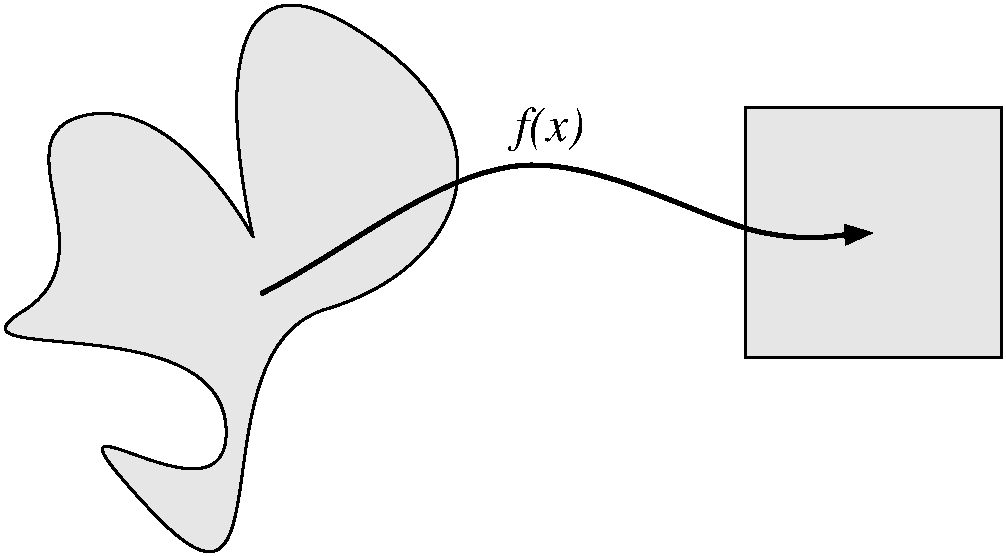
\includegraphics[scale=0.3]{figs/simpledia.pdf}
\caption{The function $f$ takes the points in the region on the right and maps them to the rectangular region.}
\label{simpledia}
\end{figure}



In order to do this we use a method from complex analysis called the \sch mapping. This takes some arbitrary polygon and maps it to the upper half-plane ($H^+$) or the unit disk. This is achieved in the $H^+$ case by taking the vertices of the polygon and mapping them to points on the real line (see fig. \ref{reallinedia}.) For the unit disk case, we look for points on the circle bounding the unit disk and which vertices they map to on the polygon (see fig. \ref{unitdiskdia}.)

% Diagram showing upper half plane to polygon
\begin{figure} [tbp]
\centering
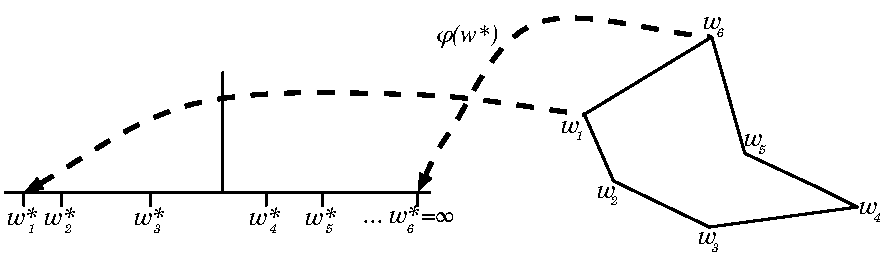
\includegraphics[scale=0.6]{figs/reallinedia.pdf}
\caption{Here we show the mapping of the upper half-plane to the polygon. The vertices ($w_i$) are the result of applying $f$ to the points on the real line ($z_i$). This boundry of the polygon is mapped to the real line.}
\label{reallinedia}
\end{figure}

% Diagram showing unit disk to polygon
\begin{figure} [tbp]
\centering
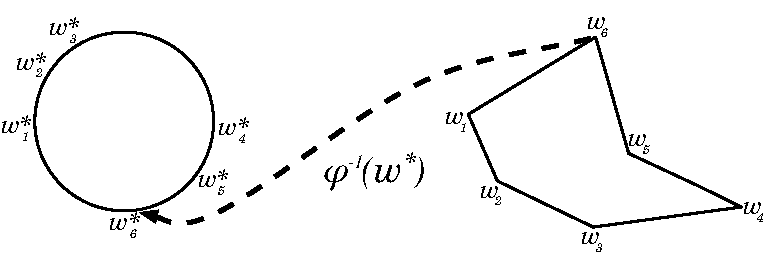
\includegraphics[scale=0.6]{figs/unitdiskdia.pdf}
\caption{We now have the same situation as in fig. \ref{reallinedia}, except that now the boundry of the polygon is mapped to the boundry of the unit disk.}
\label{unitdiskdia}
\end{figure}




Although the \sch mapping is intended for use with polygons, it is easy to take an artibrary bounded region and draw a polygon around it. This can be done either by eye (for example, using the \texttt{locator()} function in \textbf{R}) or by using a an automated process.


\subsection{Nomenclature}

We first define a polygon formally and it's associated quantities as it will be referred to throughout the rest of the document.

A polygon, $\Gamma$, is a collection of vertices $w_1, w_2,\dots,w_n$ and interior angles $\alpha_1\pi, \alpha_2\pi, \dots, \alpha_n\pi$. For convenience we define $w_{n+1} = w_1$ and $w_0=w_n$. The $w_i$ lie in $\mathbb{C} \cup {\infty}$. Numbering of vertices is counterclockwise (ie. the polygon is "to the left" as one traverses $w_k$ to $w_{k+1}$. The angles are such that $\alpha_k \in (0,2]$ and we require:

\begin{equation}
\sum_{k=1}^n (1-\alpha_k) = 2.
\end{equation}

We also define the exterior angle, $\beta_k\pi$, as given by $(1-\alpha_k)\pi$ (see fig. \ref{anglediagram}.)

% Diagram showing unit disk to polygon
\begin{figure} [tbp]
\centering
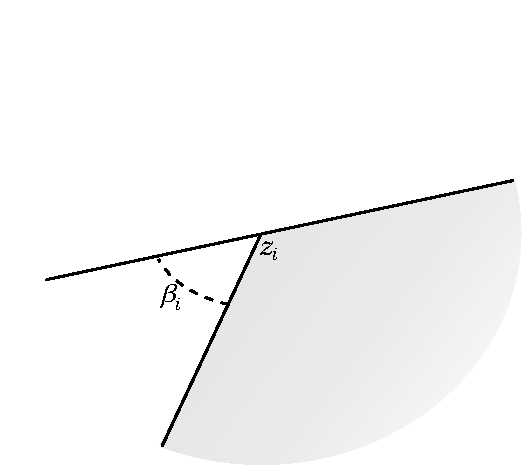
\includegraphics[scale=0.6]{figs/anglediagram.pdf}
\caption{The external angle $\beta_k$ is associated with the vertex $w_k$. The internal angle is given by $\alpha_k$.}
\label{anglediagram}
\end{figure}


Usually, $\Gamma$ is used to refer to the boundary of the polygon and $P$ to the region inside.


Since in the \sch transform we are actually looking for the inverse of the map from the polygon to the plane (or disk). We use the function $f$ to go from the unit disk or $H^+$ to the polygon and $f$s inverse, $F$ to go from the polygon to the disk or half-plane.  

We need to know the position that the vertices on $\Gamma$ (the $w_k$s) correspond to on the real line (or the boundry of the unit disk). These points are referred to as \emph{prevertices} and are denoted $z_k$.

It is certainly worth noting at this point (to avoid confusion) that those points on the polygon are always referred to as $w_i$ (for some $i$) and those on the unit disk or $H_+$ as $z_i$ (for some $i$.)



 
\section{\sch Mapping}

The \sch mapping is defined in the following way:


\begin{equation}
f(z) = A + C \int^z \prod_{k=1}^{n-1} (\zeta-z_k)^{-\beta_k} d\zeta,
\end{equation}

where $A$ and $C$ are complex constants. This is known as the \emph{\sch formula} for the half-plane.




\subsection{Mapping to the upper half-plane}

When we map $P$ to $H^+$ we set $f(\infty) = w_n$ without any loss of generality. We then have the formula (as above):

\begin{equation}
f(z) = A + C \int^z \prod_{k=1}^{n-1} (\zeta-z_k)^{-\beta_k} d\zeta.
\end{equation}



\subsection{Unit disk}

For the unit disk we do not fix any points, however note below that the product now runs over all of the prevertices. The integrand is simply a constant multiple of the original form. This is merely to avoid problems in the calculation of the branch cuts (\cite{driscoll}, \emph{p. 12}).

\begin{equation}
\label{unitscmap}
f(z) = A + C \int^z \prod_{k=1}^{n} (1 - \frac{\zeta}{z_k})^{-\beta_k} d\zeta.
\end{equation}


%\section{Special cases}




\section{Computation of the \sch mapping}

It is generally easier to compute the \sch map to the unit disk rather than to $H^+$. For that reason we only address mappings from/to the unit disk here. We now detail the process for computing the map as well as covering some of the pitfalls which may occur when computing the map.

To compute the map, we use an iterative routine to solve, numerically, the following set of equations:

\begin{equation}
\label{optimizeme}
\frac{\vert \int_{z_j}^{z_{j+1}} f^\prime(\zeta) d\zeta \vert}{\vert \int_{z_2}^{z_{1}} f^\prime(\zeta) d\zeta\vert} - \frac{\vert w_{j+1} - w_j\vert}{\vert w_2 - w_1\vert} = 0, \qquad \text{for } j=2,3,\dots,n-2,
\end{equation}

Where $f$ is as in (\ref{unitscmap}).

This set of equations should be fairly intuitive since we are just looking at the differences between the actual distances between the $w$s and those given by the current set of parameters in the current approximation for $f$.

Note that the relation does not include the vertex $w_n$, nor do we look at $w_1$ or $w_2$ in the numerator on the right of the above equation. This is since (by theorem 3.1 of \cite{driscoll} \emph{p. 24}) a polygon is precisely defined by its angles and its vertices not including $w_n$. We may also assume that up to scaling and rotation that $w_1$ and $w_2$ are correct (which is compensated for by thye complex constants.)

So, we proceed in estimating $A$, $C$ and $w_i$ for $i=1,\dots,n$ using a quasi-Newton solver\footnote{We actually use steepest descent in the early iterations, followed by Newton's method later.}. In order to calculate the integrals in (\ref{optimizeme}) we use the Guass-Jacobi quadrature.

In the software \texttt{SCPACK}\footnote{Available from \url{http://netlib.org/conformal/scpack} and \url{http://netlib.org/conformal/sclib}} written by Trefethen, the following steps are taken to compute the map (\cite{scdoc}):

\begin{enumerate}
\item Subroutine \texttt{QINIT} is called to compute Gauss-Jacobi quadrature.
\item Subroutine \texttt{SCSOLV} is called to compute the prevertices and complex onstants in the \sch mapping.
\item Subroutine \texttt{WSC} or \texttt{ZSC} is called to compute the forwards or backwards map for a series of points.
\end{enumerate}

We now address each of these steps in more detail.

\subsection{\texttt{QINIT}}

Here we set up the nodes and weights in the Gauss-Jacobi quadrature used to evaluate the integrals in \texttt{SCSOLV}. The Gauss-Jacobi quadrature is given by the following formula:

\begin{equation}
\int_{-1}^{1} (1-x)^\alpha (1+x)^\beta f(x) dx = \sum_{i=0}^{n-1}h_if(x_i) + \epsilon_n,
\end{equation}

where the $h_i$s are weights and the $x_i$ are referred to as nodes. $E_n$ is an error term. The integral is rescaled to be over the correct interval (\cite{trefethen}, \emph{p. 11}). We do not go into any further detail and treat this process as a ``black box''.

\subsection{\texttt{SCSOLV}}

The routine \texttt{SCSOLV} does the main work in finding the parameters (prevertices) of $f$. Using the nodes and weights for the Gauss-Jacobi quadrature found by \texttt{QINIT}. We then iterate through possible values for the prevertices in (\ref{unitscmap}) in order to minimise the result of the left hand side of (\ref{optimizeme}).

\subsection{\texttt{WSC} and \texttt{ZSC}}

\subsubsection{Forwards map}

Calculating the forwards map (\texttt{WSC}) is simply a case of evaluating $f$ at the necessary points. For clarity if we wish to find the point on polygon ($w$) given we know the point on the disk ($z$) we compute:

\begin{equation}
\label{unitscmap}
w=f(z) = w_0 + C \int_{z_0}^{z} \prod_{k=1}^{n} (1 - \frac{\zeta}{z_k})^{-\beta_k} d\zeta,
\end{equation}

where $z_0$ is any point in the closed disk such that $w_0 = f(z_0)$ is known and non-infinite. We may choose any point since the integrand is analytic throughout the mapping and hence the integral is path-independent (\cite{driscoll} \emph{p. 27}).


\subsubsection{Backwards map}

To calculate points from the polygon to points on the unit disk, we treat the equation $w(z)=w$ as a non-linear equation to be solved for $z$ (\cite{trefethen}, \emph{pp. 16-17}). These are solved iteratively as a series of first order ODEs, with the starting values coming from inverting (\ref{unitscmap}).



\section{Application to finite area smoothing}

Given some complex geographical area, it is possible to find a polygonal ``bounding box'' that may be fed into the \sch formula. We would then have the region transformed into the  unit disk which would not include any peninsula or other geographical features which are hard to smooth over.

Once $f$ is found, it would simply be a case of feeding all calculations through it to find the transformed co-ordinates on the unit disk. Once the smooth has been fit the area could be back-transformed and then the smooth used as usual.

This is a test.





\bibliographystyle{plainnat}
\bibliography{sc-refs}

\end{document}
